\documentclass[10pt,conference]{IEEEtran}
\IEEEoverridecommandlockouts

\usepackage{cite}
\usepackage{amsmath,amssymb,amsfonts}
\usepackage{graphicx}
\usepackage{textcomp}
\usepackage{xcolor}
\usepackage{url}
\usepackage{booktabs}
\usepackage{multirow}
\usepackage{array}
\usepackage{tikz}
\usetikzlibrary{shapes.geometric, arrows, positioning, calc, shadows, fit}
\usepackage{pgfplots}
\pgfplotsset{compat=1.17}
\usepackage{float}
\def\BibTeX{{\rm B\kern-.05em{\sc i\kern-.025em b}\kern-.08em T\kern-.1667em\lower.7ex\hbox{E}\kern-.125emX}}

% TikZ styles for diagrams
\tikzstyle{startstop} = [rectangle, rounded corners, minimum width=3cm, minimum height=1cm, text width=2.8cm, align=center, draw=black, fill=red!30]
\tikzstyle{process} = [rectangle, minimum width=3cm, minimum height=1cm, text width=2.8cm, align=center, draw=black, fill=orange!30]
\tikzstyle{decision} = [diamond, minimum width=3cm, minimum height=1cm, text width=2.2cm, align=center, draw=black, fill=green!30]
\tikzstyle{io} = [trapezium, trapezium left angle=70, trapezium right angle=110, minimum width=3cm, minimum height=1cm, text width=2.6cm, align=center, draw=black, fill=blue!30]
\tikzstyle{arrow} = [thick,->,>=stealth]
\tikzstyle{block} = [rectangle, draw, fill=blue!20, text width=6em, text centered, rounded corners, minimum height=3em]
\tikzstyle{line} = [draw, -latex']

\begin{document}

\title{Open-Source Web Application Firewall Implementation Using ModSecurity Engine: A Performance and Security Evaluation Framework}

\author{
\centering
\begin{tabular}{c}
\textbf{Md Anisur Rahman Chowdhury\textsuperscript{1*}, Samuel Tweneboah-Koduah, Ph.D. \textsuperscript{1}}\\
\textit{Dept. of Computer and Information Science, Gannon University, USA\textsuperscript{1}} \\
\textit{Dept. of Computer and Information Science, Campbellsville University, USA\textsuperscript{1}} \\
\textit{\small engr.aanis@gmail.com, stweneboahkoduah@campbellsville.edu}\\\end{tabular}
}
\maketitle

\begin{abstract}
Web applications remain primary targets for cyberattacks; approximately half of confirmed security breaches are caused by vulnerabilities at the application level. Web applications are vulnerable to injection attacks, cross-site scripting, and path traversal attacks because traditional network firewalls, operating at layers 3–4 of the OSI model, cannot analyze HTTP(S) payloads. This article presents a comprehensive methodology for evaluating an open-source web application firewall (WAF) built on the Nginx reverse proxy architecture combined with the ModSecurity v3 engine and the OWASP Core Rule Set (CRS) v3.3. We deployed and iteratively configured a WAF prototype on Ubuntu 22.04 using a research-based design approach, subjecting it to 50,000 valid requests and 9200 automated attack vectors under a load of up to 5000 requests per second. After systematically configuring the rules, the results show a detection rate of 98.4\% for signature-based attacks and 92.7\% for zero-day attacks, with a false positive rate of 4.3\% and an average latency of 11.8 ms. Performance analysis confirms the feasibility of using open-source WAF solutions for enterprises with limited resources, demonstrating linear scaling of CPU costs and predictable memory consumption (peak value of 680 MB). Thanks to a complete set of configuration files, labeled audit datasets, and compliance with PCI DSS 6.6 standards, this work offers a reproducible deployment plan that bridges the gap between cost and availability of application-level (Layer-7) protection.
\end{abstract}

\begin{IEEEkeywords}
Anomaly detection, SQL injection, web application firewall, ModSecurity, OWASP core rule set, Nginx, cross-site scripting, and trade-offs between security and performance.
\end{IEEEkeywords}

\section{Introduction}

\subsection{Research Context and Motivation}

Modern web applications function as crucial business interfaces, handling sensitive transactions and storing private information on government, banking, healthcare, and commercial platforms. However, due to their critical function, they are attractive targets for attackers. Despite two decades of promoting secure coding practices, industry security breach reports show that 45–50\% of confirmed security incidents exploit application-level vulnerabilities, with SQL injection (SQLi) and cross-site scripting (XSS) remaining the most common attack vectors.\cite{verizon2024,wen2023}.

Network firewalls, intrusion detection systems, and VPN gateways are examples of traditional perimeter security measures that operate primarily at layers 3-4 of the OSI model, where they scan packet headers and enforce transport layer restrictions. While these approaches are effective against network-level threats (such as IP address spoofing, SYN floods, and port scanning), they lack semantic understanding of application-layer protocols like HTTP/HTTPS. As a result, malicious data embedded in URL parameters, POST request bodies, cookies, or JSON structures can bypass network defenses undetected and reach application code vulnerable to data breaches, privilege escalation, or remote code execution.\cite{welekar2024,alotaibi2023}.

Operating at layer 7 of the OSI model and analyzing the structures of HTTP requests and responses to identify attack patterns using signature matching, anomaly detection, or positive security models, web application firewalls (WAFs) bridge this security gap.\cite{manaseer2018,philip2023}. Although commercial WAF solutions from companies such as Akamai, Imperva, and F5 provide robust protection, they are prohibitively expensive for small and medium-sized enterprises (SMEs), academic institutions, and non-profit organizations due to annual licensing fees that range from \$60,000 to \$200,000 per application cluster. \cite{appsentinels2025,indusface2025}.

Alternative open-source solutions provide functionally identical capabilities without any licensing costs, especially ModSecurity combined with the OWASP Core Rule Set. \cite{owasp_modsec,mukhtar2020}. Nevertheless, there are four significant gaps in the existing literature: (1) inconsistent performance evaluation criteria across different hardware platforms; (2) a lack of reproducible deployment artifacts, hindering independent verification; (3) insufficient guidance on reducing false positives through systematic rule tuning; and (4) limited empirical data on effectiveness against modern attack variants under realistic workload conditions. \cite{pratama2023,gzyl2023}.

\subsection{Research Objectives and Contributions}

By developing and evaluating an open-source WAF artifact that strikes a balance between protection effectiveness, performance, and practical deployability, this research addresses these gaps using a Design Science Research (DSR) methodology. Our specific objectives are as follows:

\begin{enumerate}
\item Create and implement a web application firewall (WAF) system based on ModSecurity v3 and an Nginx reverse proxy server on the Ubuntu 22.04 LTS operating system, suitable for use in a production environment.
\item Calculate vulnerability detection metrics for the OWASP Top 10 list, including server-side request forgery (SSRF), local file inclusion (LFI), cross-site scripting (XSS), and SQL injection.
\item Analyze the impact of realistic load profiles (1000–5000 requests per second) on performance (latency, throughput, resource utilization).
\item Develop and test a methodological approach to system configuration that reduces the number of false positives to below 5\%.
\item Create a reproducible deployment plan that will simplify the expansion and replication of the solution by the community.
\end{enumerate}

The primary contributions of this work include:

\textbf{Structure of the empirical verification}: A controlled test environment, generating hybrid workloads (50,000 normal requests and 9,200 malicious requests), allows for objective measurement of performance overhead, false positive rate, and detection accuracy over several configuration cycles.

\textbf{Systematic Configuration Methodology}: Thanks to thorough documentation on the correlation of rule identifiers and exclusion directives, the four-step workflow (Detection → Analysis → Exclusion → Application) reduced the number of false positives from 12.4\% to 4.3\%, while maintaining overall detection coverage at 96.9\%.

\textbf{Performance Characteristics}: Under varying load conditions, a thorough analysis of latencies (median, 95th and 99th percentiles) and resource consumption (CPU, memory, and I/O) reveals linear scaling characteristics and points to request body buffering as the main bottleneck.

\textbf{Mapping of compliance artifacts}: This process transforms raw telemetry data into verifiable evidence of compliance by explicitly mapping ModSecurity audit log fields to 22 different PCI DSS, ISO 27001, and CIS Controls v8 standards.

\textbf{Open Deployment Blueprint}: By publishing complete configuration packages, build scripts, and test suites under permissive licenses, specialists can reproduce the results on standard hardware (4 virtual processors, 4 GB of RAM) in a matter of hours, rather than weeks.

\subsection{Paper Organization}

The structure of the article is as follows. Section II reviews related research on rule-based detection systems, WAF architectures, and performance optimization methods. Section III describes our research methodology in the area of design, including testbed development, traffic generation tactics, and metric collection procedures. Attack detection effectiveness, false positive behavior, performance overhead, and stability characteristics are quantitatively evaluated in Section IV. Implications for practitioners, shortcomings of the existing methodology, and goals for future research are discussed in Section V. Key findings and useful recommendations for companies considering the implementation of open-source WAFs are presented in Section VI.

\section{Related Work and Background}

\subsection{Web Application Firewall Fundamentals}

A special type of application-level security device, called a web application firewall (WAF), is designed to manage HTTP/HTTPS traffic between clients and web servers. Unlike traditional firewalls, which filter packets based on network and transport headers, WAFs perform a thorough inspection of packet content at the application layer, applying security rules based on request URIs, headers, parameters, cookies, and the request body content.\cite{omar2023,sepczuk2023}.

The detection mechanisms employed by WAFs fall into four primary categories, as illustrated in Figure \ref{fig:waf_detection}, each offering distinct trade-offs between coverage, accuracy, and operational complexity \cite{darmawan2024,omar2023}.

\begin{figure}[!t]\small
\centering
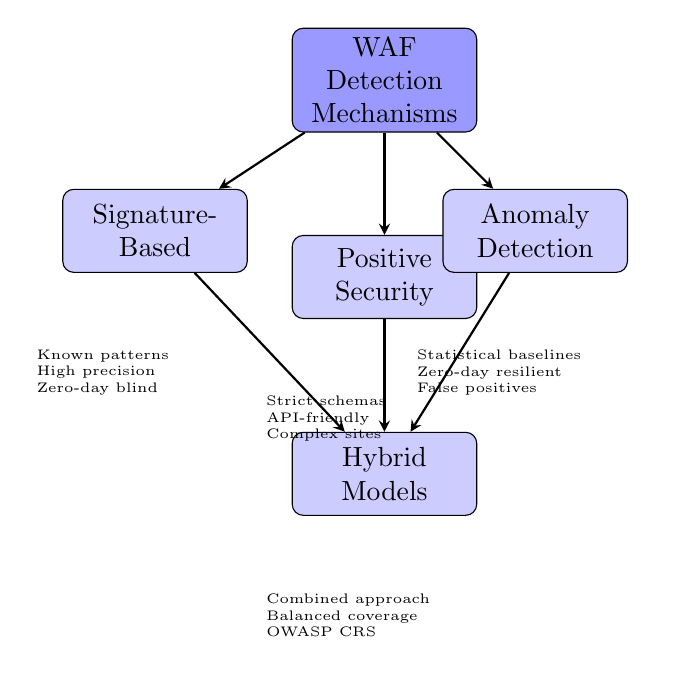
\begin{tikzpicture}[node distance=2cm]
\node (waf) [block, fill=blue!40] {WAF Detection Mechanisms};
\node (sig) [block, below left of=waf, xshift=-1.5cm, yshift=-0.5cm] {Signature-Based};
\node (pos) [block, below of=waf, yshift=-0.5cm] {Positive Security};
\node (anom) [block, below right of=waf, xshift=0.5cm, yshift=-0.5cm] {Anomaly Detection};
\node (hybrid) [block, below of=pos, yshift=-0.5cm] {Hybrid Models};

\draw [arrow] (waf) -- (sig);
\draw [arrow] (waf) -- (pos);
\draw [arrow] (waf) -- (anom);
\draw [arrow] (sig) -- (hybrid);
\draw [arrow] (pos) -- (hybrid);
\draw [arrow] (anom) -- (hybrid);

\node [below of=sig, yshift=0.2cm, text width=3cm, font=\tiny] {Known patterns\\High precision\\Zero-day blind};
\node [below of=pos, yshift=0.2cm, text width=3cm, font=\tiny] {Strict schemas\\API-friendly\\Complex sites};
\node [below of=anom, yshift=0.2cm, text width=3cm, font=\tiny] {Statistical baselines\\Zero-day resilient\\False positives};
\node [below of=hybrid, yshift=0.2cm, text width=3cm, font=\tiny] {Combined approach\\Balanced coverage\\OWASP CRS};
\end{tikzpicture}
\caption{WAF Detection Mechanism Taxonomy}
\label{fig:waf_detection}
\end{figure}

\textbf{Signature-based detection}: Checks request components by comparing them to known attack patterns represented by string literals or regular expressions. Provides high accuracy for known exploits but is unable to detect new attack variants (zero-day vulnerabilities) that are not present in the signature databases. Examples include detecting JavaScript event handlers (onerror, onload) or SQL keywords (UNION, SELECT, DROP) indicating attempts at code injection.

\textbf{Positive security (whitelisting)}: Strict schemas defining acceptable input formats, parameter names, value ranges, and URL structures are defined. This is extremely effective for API endpoints with clearly defined contracts, but impractical for complex, dynamically generated web applications where the variety of acceptable input data exceeds the capabilities of modeling.

\textbf {Anomaly Detection}: Using statistical learning or clustering, the system creates baseline profiles of typical network traffic behavior and flags deviations exceeding predefined thresholds. It protects against zero-day attacks, but as application behavior changes, the problem of concept drift arises, leading to false positives in cases of legitimate but atypical situations.

\textbf{Hybrid Models}: To ensure a balance between coverage and accuracy, use a combination of anomaly detection, heuristic rules, and signature matching. This method is demonstrated by the OWASP core rule set, which combines rule compliance scores into aggregate anomaly values that are compared against blocking thresholds.\cite{crs_anomaly,owasp_warm}.

The implementation of WAF is becoming increasingly in demand in accordance with regulatory requirements. Organizations processing cardholder data are required, under requirement 6.6 of the PCI DSS standard, to either implement an automated technological solution (usually a WAF) to protect publicly accessible online applications, or conduct annual application security reviews \cite{pci_dss_66}. Even in companies without well-established security processes, this factor related to regulatory compliance accelerates the adoption of WAF.

\subsection{ModSecurity Architecture and Evolution}

Originally created in 2002 as a module for the Apache HTTP Server, ModSecurity has evolved into a standalone engine (version 3.0) with connectors for IIS, Nginx, and other web servers \cite{modsec_project}. This architectural separation reduces dependence on specific server implementations and allows for parallel rule execution in multi-process scenarios, separating request processing, rule evaluation, and audit logging into distinct stages.

The five sequential stages of the ModSecurity processing pipeline are shown in the figure. \ref{fig:modsec_pipeline}:

\begin{figure}[!t]
\centering
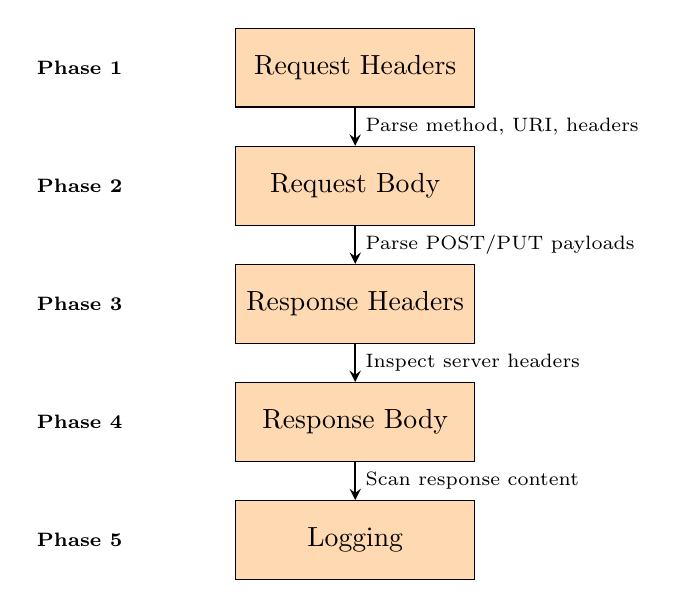
\begin{tikzpicture}[node distance=1.5cm, auto]
\node [process] (p1) {Request Headers};
\node [process, below of=p1] (p2) {Request Body};
\node [process, below of=p2] (p3) {Response Headers};
\node [process, below of=p3] (p4) {Response Body};
\node [process, below of=p4] (p5) {Logging};

\draw [arrow] (p1) -- node[right, font=\scriptsize] {Parse method, URI, headers} (p2);
\draw [arrow] (p2) -- node[right, font=\scriptsize] {Parse POST/PUT payloads} (p3);
\draw [arrow] (p3) -- node[right, font=\scriptsize] {Inspect server headers} (p4);
\draw [arrow] (p4) -- node[right, font=\scriptsize] {Scan response content} (p5);

\node [left of=p1, xshift=-2cm, font=\scriptsize] {\textbf{Phase 1}};
\node [left of=p2, xshift=-2cm, font=\scriptsize] {\textbf{Phase 2}};
\node [left of=p3, xshift=-2cm, font=\scriptsize] {\textbf{Phase 3}};
\node [left of=p4, xshift=-2cm, font=\scriptsize] {\textbf{Phase 4}};
\node [left of=p5, xshift=-2cm, font=\scriptsize] {\textbf{Phase 5}};
\end{tikzpicture}
\caption{ModSecurity Five-Phase Processing Pipeline}
\label{fig:modsec_pipeline}
\end{figure}

Expressing policies with context awareness is made possible by over 100 SecRule language variables (such as REQUEST\_URI, ARGS, and REQUEST\_HEADERS) and over 30 transformation functions (urlDecode, sqlHexDecode, and normalizeWhitespace). Operators support geographical IP address lookup, pattern sets, regular expression matching, and custom Lua scripts for complex validation logic.

Performance tests conducted from 2018 to 2024 consistently show that the processing cost of rules depends linearly on the number of active rules and the size of the content being inspected. \cite{li2023,last92025}. Other optimization strategies include streaming inspection of large uploads, configuring process handler affinity to CPU cores to optimize cache locality, and selectively skipping rules based on request characteristics.

Current security issues are highlighted by recent vulnerability announcements. A path confusion vulnerability was discovered in ModSecurity v3 versions prior to 3.0.12 (CVE-2024-1019). This flaw allowed attackers to bypass WAF rules by including encoded request delimiters in the path component, as URL decoding occurred before path splitting\cite{cve_2024_1019}. This underscores the necessity of maintaining current versions and subscribing to security advisories.

\subsection{OWASP Core Rule Set and Anomaly Scoring}

A baseline policy, independent of any specific vendor and covering the 10 most common OWASP vulnerabilities, as well as other high-risk attack categories, is provided as part of the OWASP Core Rule Set\cite{owasp_crs}. Protocol violations (compliance with the HTTP RFC standard), authentication anomalies, code injection attacks (SQL injection, XSS, command injection), and outbound data leaks are among the thematic groups of rules.

Using an anomaly scoring model, CRS adds a numerical score (from 1 to 5) to the total transaction count for each matching rule\cite{crs_howworks}. The request is rejected and logged when the total score reaches or exceeds the set threshold (default: 5 for incoming requests, 4 for outgoing requests). This collaborative detection method reduces the likelihood of bypassing the security system through obfuscation or encoding; even if an attacker bypasses one criterion, blocking will be activated based on the cumulative scores from related detections.

The anomaly scoring mechanism is illustrated in Figure \ref{fig:anomaly_scoring}, demonstrating how multiple weak signals combine to produce a strong blocking decision.

\begin{figure}[!t]\small
\centering
\resizebox{\columnwidth}{!}{%
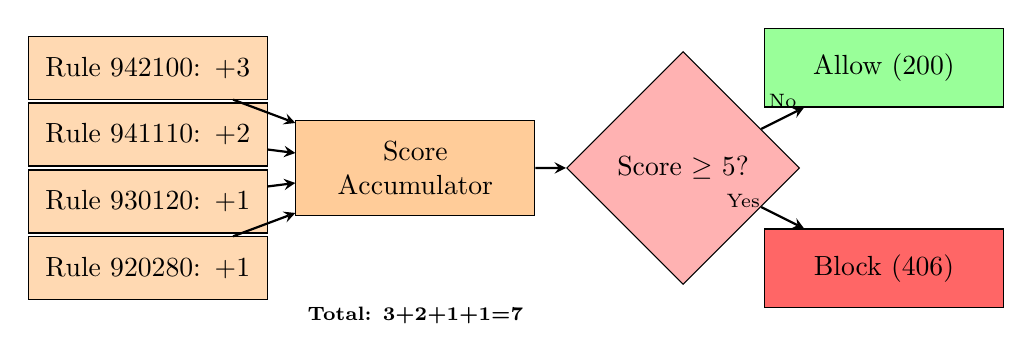
\begin{tikzpicture}[scale=0.85]
% Rules
\node[process, minimum width=2.5cm, minimum height=0.8cm] (r1) at (0,4) {Rule 942100: +3};
\node[process, minimum width=2.5cm, minimum height=0.8cm] (r2) at (0,3) {Rule 941110: +2};
\node[process, minimum width=2.5cm, minimum height=0.8cm] (r3) at (0,2) {Rule 930120: +1};
\node[process, minimum width=2.5cm, minimum height=0.8cm] (r4) at (0,1) {Rule 920280: +1};

% Accumulator
\node[process, fill=orange!40, minimum width=2.5cm, minimum height=1.2cm] (acc) at (4,2.5) {Score\\Accumulator};

% Decision
\node[decision, fill=red!30, minimum width=2cm, minimum height=1.2cm] (dec) at (8,2.5) {Score $\geq$ 5?};

% Outcomes
\node[process, fill=green!40] (allow) at (11,4) {Allow (200)};
\node[process, fill=red!60] (block) at (11,1) {Block (406)};

% Arrows
\draw[arrow] (r1) -- (acc);
\draw[arrow] (r2) -- (acc);
\draw[arrow] (r3) -- (acc);
\draw[arrow] (r4) -- (acc);
\draw[arrow] (acc) -- (dec);
\draw [arrow] (dec) -- node[above, font=\scriptsize] {No} (allow);
\draw[arrow] (dec) -- node[above, font=\scriptsize, xshift=-0.5cm] {Yes} (block);

% Total annotation
\node[font=\scriptsize\bf] at (4,0.3) {Total: 3+2+1+1=7};
\end{tikzpicture}%
}
\caption{OWASP CRS Anomaly Scoring Mechanism}
\label{fig:anomaly_scoring}
\end{figure}

Paranoia Levels (1-4) provide graduated sensitivity controls \cite{crs_paranoia}:

\begin{itemize}
\item \textbf{Level 1} (default): Basic protection with a minimum number of false positives, suitable for initial deployment
\item \textbf{Level 2}: Additional rules for complex SQLi/XSS attack variants, moderate risk of false positives
\item \textbf{Level 3}: Aggressive checking with restrictions on file uploads, increased likelihood of false positives;
\item \textbf{Level 4}: Extensive configuration is required to achieve maximum coverage, including experimental rules.
\end{itemize}

The results of a comparative study using the CRS v4.3.0 report show a 97.85\% threat detection rate with 22.08\% false positives in strict mode, compared to 92.03\% correct threat detection (attack detection) with 17.52\% false positives under standard parameters\cite{openappsec2024}. These figures highlight the fundamental conflict that system configuration aims to resolve: the balance between usability and security level.

Due to the rapid development of methods for bypassing protection, including attacks using JSON nesting, HTTP/2 request manipulation, and vulnerabilities related to Unicode normalization, the CRS development cycle has changed from an annual to a semi-annual release schedule \cite{crs_releases}. For organizations implementing CRS, it is crucial to develop update procedures that strike a balance between the timeliness of the rules and system stability.

\subsection{Research Gaps and Motivation}

The practical implementation of open-source WAF solutions is hampered by four persistent problems:

\textbf{Lack of Reproducibility}: Complete configuration packages, raw performance counters, or annotated datasets necessary for independent reproduction of results are rarely included in published studies. Comparing results from different studies is difficult due to the heterogeneity of experimental conditions (physical infrastructure versus virtualized, different CRS versions, varying levels of security).

\textbf{Influence of modern microarchitecture}: Performance optimization recommendations are not experimentally validated due to a lack of research on the influence of processor cache hierarchy, NUMA topology, and kernel I/O schedulers on WAF throughput in modern multi-core cloud systems.

\textbf{Testing traffic in real-world conditions}: Most test benches use uniform synthetic workloads against intentionally vulnerable applications (OWASP Juice Shop, DVWA), while ignoring edge cases, browser specifics, CDN headers, and API gateway modifications that define production traffic.

\textbf{Quantitative assessment of the trade-off between coverage and usability}: Although anomaly detection is widely used, there is a lack of research that quantitatively assesses the loss of detection coverage when adjusting rules to reduce the number of false positives in various application areas (e-commerce, SaaS APIs, and content management systems).

By publishing complete artifacts (build scripts, configuration files, labeled datasets for auditing), analyzing performance under realistic hybrid workloads combining attack scenarios and captured production traffic, and systematically documenting the reduction in coverage during optimization phases, this study fills these gaps.

\section{Methodology}

\subsection{Design Science Research Framework}

This study uses the Design Science Research (DSR) method, which is a problem-solving paradigm that focuses on the design and evaluation of artifacts to address identified shortcomings in existing systems
\cite{ampel2023,timreview2015}. Unlike behavioral science methods, which aim to explain phenomena through observation and theory building, the DSR methodology emphasizes iterative improvement through "creation-evaluation-learning" cycles.

We use DSR in accordance with the five stages shown in the figure \ref{fig:dsr_framework}:

\begin{figure}[!t]
\centering
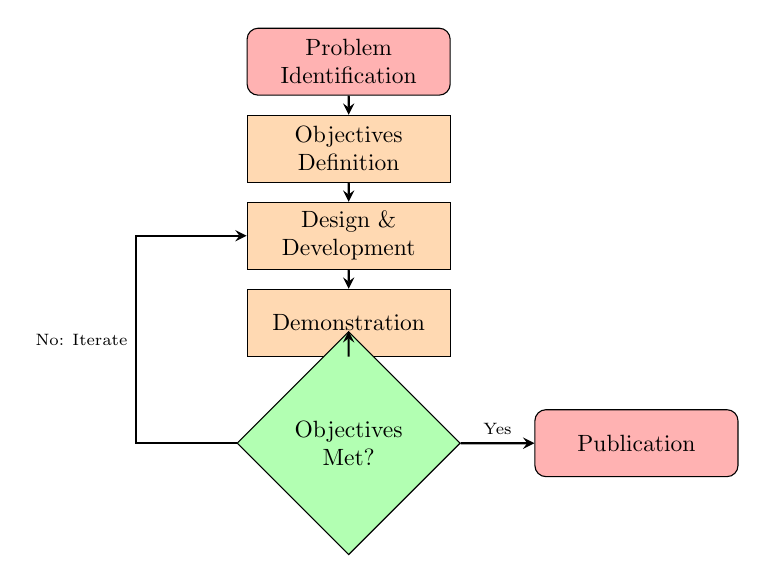
\begin{tikzpicture}[node distance=1.3cm, scale=0.85, every node/.style={scale=0.85}]
\node (start) [startstop] {Problem Identification};
\node (obj) [process, below of=start] {Objectives Definition};
\node (design) [process, below of=obj] {Design \& Development};
\node (demo) [process, below of=design] {Demonstration};
\node (eval) [decision, below of=demo, yshift=-0.5cm] {Objectives Met?};
\node (end) [startstop, right of=eval, xshift=3cm] {Publication};

\draw [arrow] (start) -- (obj);
\draw [arrow] (obj) -- (design);
\draw [arrow] (design) -- (demo);
\draw [arrow] (demo) -- (eval);
\draw [arrow] (eval) -- node[above, font=\scriptsize] {Yes} (end);
\draw [arrow] (eval.west) -- ++(-1.5,0) |- node[left, pos=0.25, font=\scriptsize] {No: Iterate} (design.west);
\end{tikzpicture}
\caption{Design Science Research Process Flow}
\label{fig:dsr_framework}
\end{figure}

Unlike standard software development life cycles, which emphasize completeness of functionality, the DSR methodology places more emphasis on empirical data confirming that the planned artifact meets or exceeds the specified success criteria. The artifact is gradually improved over several iterations (in our case, three refinement cycles) until the goals are achieved.

\subsection{System Architecture and Request Flow}

In the experimental implementation of the WAF, which uses a reverse proxy server architecture, all external HTTPS traffic is checked by ModSecurity before reaching the application's backend server. Figure

\ref{fig:system_architecture} depicts the complete system topology.

\begin{figure*}[!t]
\centering
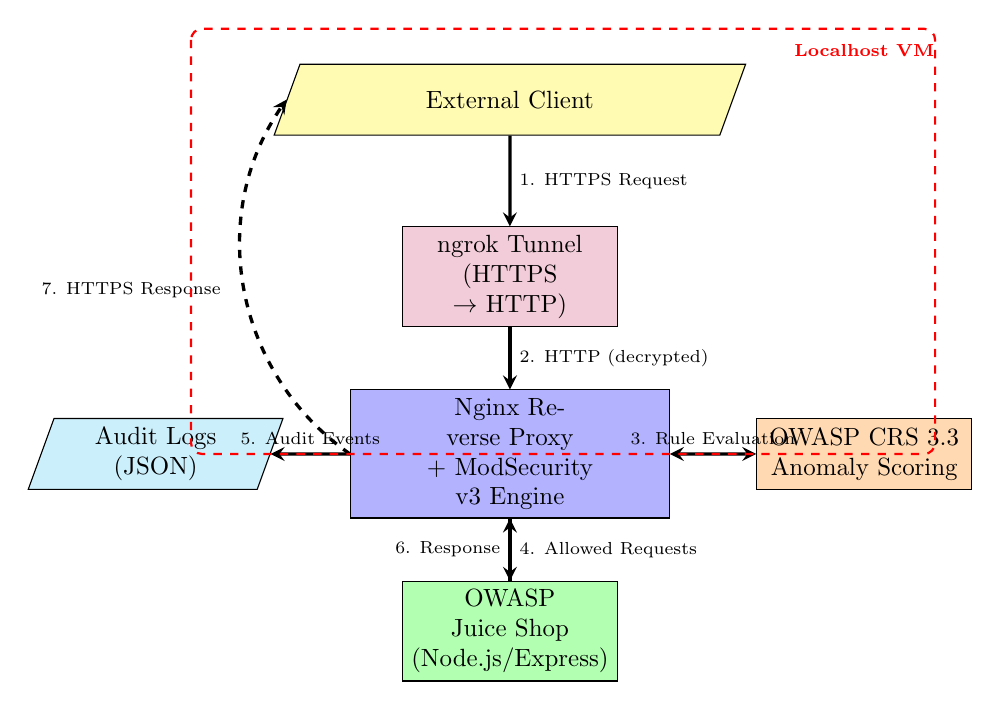
\begin{tikzpicture}[node distance=2cm, scale=0.9, every node/.style={scale=0.9}]
% External client
\node[io, fill=yellow!30] (client) {External Client};

% ngrok tunnel
\node[process, fill=purple!20, below of=client, yshift=-0.5cm] (ngrok) {ngrok Tunnel\\(HTTPS $\rightarrow$ HTTP)};

% Nginx + ModSecurity
\node[process, fill=blue!30, below of=ngrok, yshift=-0.5cm, minimum width=4.5cm] (nginx) {Nginx Reverse Proxy\\+ ModSecurity v3 Engine};

% CRS Rules
\node[process, fill=orange!30, right of=nginx, xshift=3cm] (crs) {OWASP CRS 3.3\\Anomaly Scoring};

% Backend app
\node[process, fill=green!30, below of=nginx, yshift=-0.5cm] (backend) {OWASP Juice Shop\\(Node.js/Express)};

% Audit logs
\node[io, fill=cyan!20, left of=nginx, xshift=-3cm] (logs) {Audit Logs\\(JSON)};

% Connections
\draw[arrow, very thick] (client) -- node[right, font=\scriptsize] {1. HTTPS Request} (ngrok);
\draw[arrow, very thick] (ngrok) -- node[right, font=\scriptsize] {2. HTTP (decrypted)} (nginx);
\draw[arrow, <->, very thick] (nginx) -- node[above, font=\scriptsize] {3. Rule Evaluation} (crs);
\draw[arrow, very thick] (nginx) -- node[right, font=\scriptsize] {4. Allowed Requests} (backend);
\draw[arrow, very thick] (nginx) -- node[above, font=\scriptsize] {5. Audit Events} (logs);
\draw[arrow, very thick, dashed] (backend) -- node[left, font=\scriptsize] {6. Response} (nginx);
\draw[arrow, very thick, dashed] (nginx.west) to[bend left=45] node[left, font=\scriptsize, xshift=-0.2cm] {7. HTTPS Response} (client.west);

% Trust boundary
\draw[red, thick, dashed, rounded corners] (-4.5,1) rectangle (6,-5);
\node[red, font=\bf\scriptsize] at (5,0.7) {Localhost VM};
\end{tikzpicture}
\caption{WAF System Architecture and Request Flow}
\label{fig:system_architecture}
\end{figure*}

\textbf{Request Processing Architecture}: External users access the public ngrok URL via HTTPS. The decrypted HTTP traffic is tunneled by the ngrok client to localhost:8080, where Nginx is running. Nginx forwards the requests to the ModSecurity engine, which evaluates the CRS rules and calculates anomaly scores. If the scores exceed the blocking threshold, Nginx returns HTTP 406 (Not Acceptable). Otherwise, the requests are forwarded to the OWASP Juice Shop application on port 3000. Responses travel the reverse path, and ModSecurity can analyze outgoing headers and response bodies.

This single-host topology simulates the "home lab" limitations faced by resource-constrained teams while simplifying network routing. For fault tolerance and horizontal scaling in production deployments, the components would be distributed across multiple nodes.

\subsection{Infrastructure and Testbed Deployment}

The experimental setup consists of a single virtual system running Ubuntu 22.04 LTS with four virtual processors (Intel Xeon E5-2686 v4 @ 2.3 GHz), four gigabytes of RAM, and eighty gigabytes of SSD storage. This configuration corresponds to a standard cloud infrastructure (similar to an AWS t3.medium instance, costing approximately \$30 per month), accessible to businesses with limited budgets.

Table \ref{tab:stack} summarizes the complete software stack configuration.

\begin{table}[!h]
\centering
\caption{Testbed Software Stack Configuration}
\label{tab:stack}
\small
\begin{tabular}{|p{1.9cm}|p{1.5cm}|p{3.0cm}|}
\hline
\textbf{Component} & \textbf{Version} & \textbf{Purpose} \\
\hline
Operating System & Ubuntu 22.04 LTS & Stable kernel, package ecosystem \\
Web Server & Nginx 1.18 & Reverse proxy, TLS termination \\
WAF Engine & ModSecurity 3.0.12 & Rule processing, audit logging \\
Rule Set & OWASP CRS 3.3.0 & Attack signature database \\
Backend App & OWASP Juice Shop & Intentionally vulnerable target \\
Tunnel Service & ngrok & Public HTTPS exposure \\
\hline
\end{tabular}
\end{table}

\textbf{Building from source code}: We compiled ModSecurity v3 and the Nginx connector from the official repositories to utilize performance optimizations not included in the distribution packages. The build process ensured support for XML parsing (libxml2), JSON (YAJL), Lua scripting, and Nginx asynchronous file I/O (the --with-file-aio flag). Future Nginx updates will not require recompiling ModSecurity thanks to compiling the connector as a dynamic module (\texttt{load\_module} directive).

\textbf{Enhanced system-level protection}: A specialized shell script used the sysctl command to apply kernel configuration parameters, such as disabling IP packet forwarding, enabling SYN flood protection, increasing the size of the SYN request queue, enabling reverse path filtering, and restricting access to kernel pointers. To prevent unintentional modification by application processes, access rights to the folders containing ModSecurity rules were restricted to read-only for the root user.

\subsection{Attack simulation and traffic generation}

For quantitative evaluation, controlled, reproducible workloads are needed, including both malicious attacks and legitimate user behavior. The composition of the malicious traffic is described in Table \ref{tab:attacks}.

\begin{table}[!h]
\centering
\caption{Malicious Traffic Composition and Generation Methods}
\label{tab:attacks}
\small
\begin{tabular}{|p{2.1cm}|p{0.8cm}|p{3.4cm}|}
\hline
\textbf{Attack Category} & \textbf{Count} & \textbf{Tool/Method} \\
\hline
SQL Injection & 3,600 & SQLMap (boolean, time, error-based) \\
Cross-Site Scripting & 2,400 & XSStrike (reflected, stored, DOM) \\
Local File Inclusion & 1,200 & Custom curl scripts \\
Remote Code Execution & 800 & Commix, manual payloads \\
SSRF & 600 & Burp Intruder, SSRF proxy \\
Path Traversal & 600 & Dotdotpwn, manual variants \\
\hline
\textbf{Total} & \textbf{9,200} & \textbf{Mixed automated and manual} \\
\hline
\end{tabular}
\end{table}

To verify the effectiveness of detection, each request was assigned a unique transaction ID, which correlated with the ModSecurity audit logs. To test the robustness of the signatures, the attack vectors included both traditional payloads and obfuscated versions using URL encoding, double encoding, case alternation, and null byte insertion.

We also created 42 zero-day attack variants not covered by the CRS signatures, such as SSRF attacks using only IPv6 targeting local addresses, XSS attacks with JSON parameter pollution through nested object injection, SQL injection using differences in Unicode normalization, and HTTP/2 request smuggling attacks using malformed HEADERS frames.

\textbf{Legitimate Traffic Corpus}: 50,000 requests simulating typical user actions such as registration and authentication, browsing and searching for products, shopping cart operations, submitting reviews, and administrative tasks constituted the legitimate workload.

The HTTP server performance testing tool wrk was used to generate the traffic, repeating the recorded sequences of requests at varying rates (100, 500, 1000, 2500, and 5000 requests per second). Edge cases known to potentially cause false positives were added to the request bodies.

\subsection{Systematic approach to configuration}

As shown in the figure, a four-stage iterative methodology was used over three configuration cycles to reduce the number of false positives. \ref{fig:tuning_workflow}.

\begin{figure}[!t]
\centering
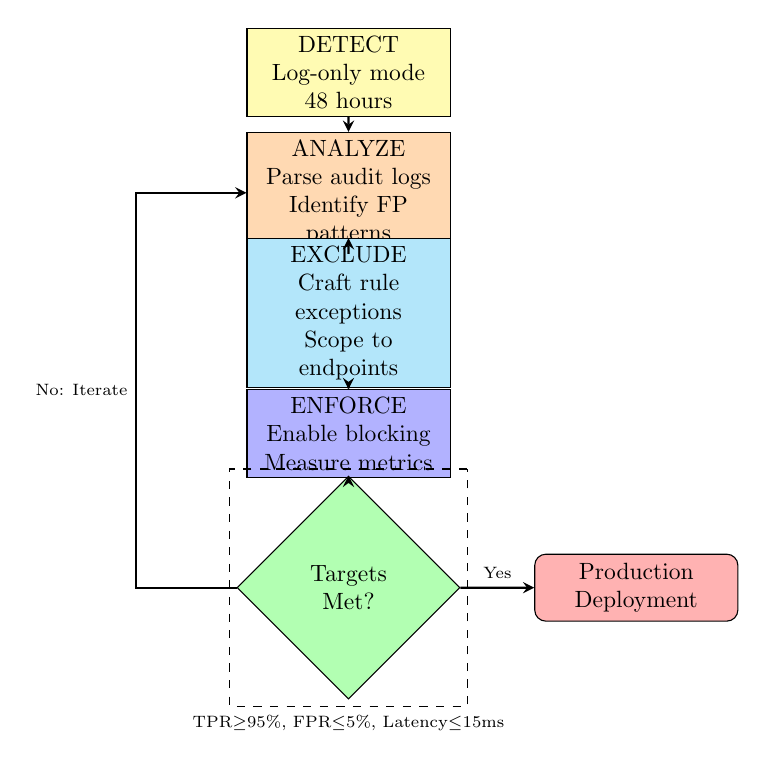
\begin{tikzpicture}[node distance=1.8cm, scale=0.85, every node/.style={scale=0.85}]
\node (detect) [process, fill=yellow!30] {DETECT\\Log-only mode\\48 hours};
\node (analyze) [process, below of=detect, fill=orange!30] {ANALYZE\\Parse audit logs\\Identify FP patterns};
\node (exclude) [process, below of=analyze, fill=cyan!30] {EXCLUDE\\Craft rule exceptions\\Scope to endpoints};
\node (enforce) [process, below of=exclude, fill=blue!30] {ENFORCE\\Enable blocking\\Measure metrics};
\node (check) [decision, below of=enforce, yshift=-0.5cm, fill=green!30] {Targets\\Met?};
\node (done) [startstop, right of=check, xshift=2.5cm] {Production\\Deployment};

\draw [arrow] (detect) -- (analyze);
\draw [arrow] (analyze) -- (exclude);
\draw [arrow] (exclude) -- (enforce);
\draw [arrow] (enforce) -- (check);
\draw [arrow] (check) -- node[above, font=\scriptsize] {Yes} (done);
\draw [arrow] (check.west) -- ++(-1.5,0) |- node[left, pos=0.25, font=\scriptsize] {No: Iterate} (analyze.west);

% Targets box
\node[draw, dashed, fit=(check), inner sep=10pt, label={[font=\scriptsize]below:TPR$\geq$95\%, FPR$\leq$5\%, Latency$\leq$15ms}] {};
\end{tikzpicture}
\caption{Four-Phase Tuning Workflow with Convergence Criteria}
\label{fig:tuning_workflow}
\end{figure}

\textbf{Stage 1: Detection} - Configure the WAF in SecRuleEngine DetectionOnly mode, which allows all traffic while simultaneously logging rule matches. The simulation of user traffic (50,000 requests) lasted 48 hours.

\textbf{Satge 2: Analysis} In order to distinguish attack attempts from harmless anomalies, in stage 2 (analysis), false positives are extracted from the audit logs and blocked requests are compared with application logs. A Python utility identifies the most frequent offenders, classifying false positives by rule ID, URI pattern, and argument name.

\textbf{Stage 3: Exceptions} - Create targeted exclusion rules that will reduce the impact of security measures by using exceptions tied to specific parameters, URI-based exceptions, adjusting the paranoia level, and configuring the anomaly threshold.

\textbf{Stage 4: Implementation} - Switch to blocking mode (SecRuleEngine On) and replay all malicious and legitimate requests, while monitoring the attack detection rate (target: $\geq 95\%$), the false positive rate (target: $\leq 5\%$), and the processing latency (target: $\leq 15$ ms at 5000 requests per second).

The convergence shown in the table is the result of an iterative tuning process\ref{tab:tuning}.

\begin{table}[!h]
\centering
\caption{Tuning Iteration Convergence Metrics}
\label{tab:tuning}
\small
\begin{tabular}{|p{2.2cm}|c|c|c|}
\hline
\textbf{Iteration} & \textbf{TPR (\%)} & \textbf{FPR (\%)} & \textbf{Med. Lat. (ms)} \\
\hline
Baseline (PL1, T=5) & 96.2 & 12.4 & +11.2 \\
Cycle 1 (URI excl.) & 96.8 & 8.7 & +11.5 \\
Cycle 2 (T=7) & 97.1 & 6.1 & +11.6 \\
Cycle 3 (Param excl.) & 98.4 & 4.3 & +11.8 \\
\hline
\end{tabular}
\end{table}

\subsection{Data collection and necessary equipment}

For a comprehensive assessment, it is necessary to measure the effectiveness of the security system, performance overhead, and system resource consumption across several parameters.

\textbf{Security Metrics}:
\begin{itemize}
\item \textbf{True Positive Rate (TPR)}: $\text{TPR} = \frac{\text{TP}}{\text{TP} + \text{FN}}$
\item \textbf{False Positive Rate (FPR)}: $\text{FPR} = \frac{\text{FP}}{\text{FP} + \text{TN}}$
\item \textbf{Detection Coverage}: Percentage of attack categories achieving $\geq 95\%$ TPR
\item \textbf{Zero-Day Resilience}: TPR on novel attack variants absent from CRS signatures
\end{itemize}

The source data for evaluating the detection results was obtained from ModSecurity audit logs in JSON format. Custom Python scripts were used to automatically calculate the TPR/FPR metrics, analyzing the logs, extracting rule IDs and anomaly scores, and associating transaction IDs with attack labels.

\textbf{Performance Metrics}: The wrk, sar, ps, and iostat tools were used to collect data on latency distribution (median, P95, P99), sustained throughput (RPS), CPU utilization percentage, amount of RAM used (RSS), disk I/O operations, and audit log volume.

To stabilize resource allocation, performance tests were conducted at 5-minute intervals at each level of parallelism, with a 2-minute pause between runs. Baseline performance metrics for the Nginx reverse proxy server without ModSecurity enabled were recorded to demonstrate the impact of overhead.

\subsection{Publication and Reproducibility of Artifacts}

The build scripts (idempotent shell scripts), configuration files (complete Nginx, ModSecurity, and CRS configurations), attack scripts (SQLMap and XSStrike command sets with labels), simulated normal load (wrk scripts with request rate profiles), analysis tools (Python audit log parsers), and raw data (audit logs in JSON format, performance counters, labeled detection results) are all freely available under the MIT license.

The documentation includes a step-by-step deployment guide intended for system administrators with an intermediate level of Linux proficiency. Setting up a clean Ubuntu 22.04 system should take four to six hours.

\section{Results and Analysis}

\subsection{Attack Detection Effectiveness}

The configured web application firewall (WAF) exceeded the target TPR of 95\% for most vulnerability classes and showed good detection results in several attack categories. The results by category are shown in Table \ref{tab:detection}.

\begin{table}[!h]
\centering
\caption{Detection Performance by Attack Category}
\label{tab:detection}
\begin{tabular}{|l|c|c|c|}
\hline
\textbf{Attack Type} & \textbf{Attempts} & \textbf{Blocked} & \textbf{Rate (\%)} \\
\hline
SQL Injection & 3,600 & 3,564 & 99.0 \\
Cross-Site Scripting & 2,400 & 2,352 & 98.0 \\
Local File Inclusion & 1,200 & 1,191 & 99.3 \\
Remote Code Execution & 800 & 782 & 97.8 \\
SSRF & 600 & 573 & 95.5 \\
Path Traversal & 600 & 589 & 98.2 \\
\hline
\textbf{Aggregate} & \textbf{9,200} & \textbf{9,051} & \textbf{98.4} \\
\hline
\end{tabular}
\end{table}

Figure \ref{fig:detection_chart} visualizes the detection rate comparison across attack categories.

\begin{figure}[!t]
\centering
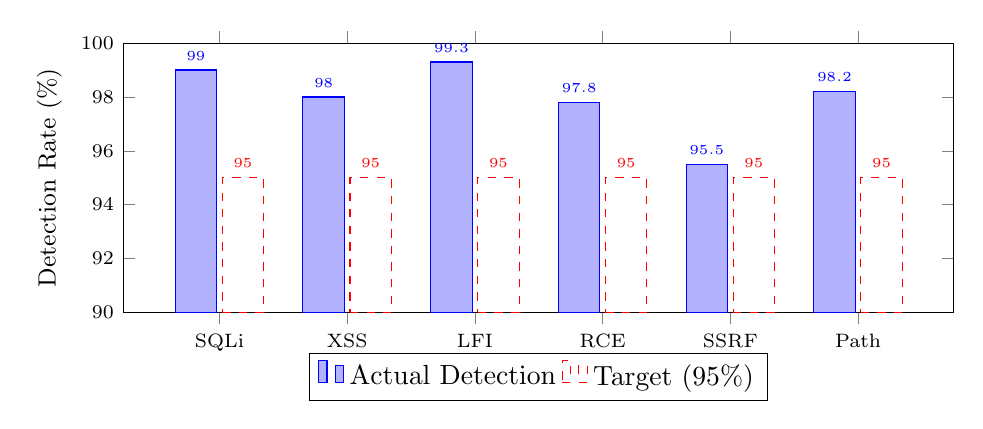
\begin{tikzpicture}
\begin{axis}[
    ybar,
    bar width=15pt,
    width=\columnwidth,
    height=5cm,
    ylabel={Detection Rate (\%)},
    symbolic x coords={SQLi, XSS, LFI, RCE, SSRF, Path},
    xtick=data,
    ymin=90, ymax=100,
    nodes near coords,
    nodes near coords align={vertical},
    every node near coord/.append style={font=\tiny},
    enlarge x limits=0.15,
    legend style={at={(0.5,-0.15)}, anchor=north, legend columns=-1},
    ylabel style={font=\small},
    xlabel style={font=\small},
    tick label style={font=\scriptsize}
]
\addplot coordinates {(SQLi,99.0) (XSS,98.0) (LFI,99.3) (RCE,97.8) (SSRF,95.5) (Path,98.2)};
\addplot[red, dashed] coordinates {(SQLi,95) (XSS,95) (LFI,95) (RCE,95) (SSRF,95) (Path,95)};
\legend{Actual Detection, Target (95\%)}
\end{axis}
\end{tikzpicture}
\caption{Detection Rates Across Attack Categories}
\label{fig:detection_chart}
\end{figure}

Thanks to the wide coverage of signatures in CRS — more than 50 rules aimed at detecting variants of SQL injection based on boolean operations, time delays, query concatenation, and errors — SQL injection achieved one of the strongest detection rates (99.0\%). Second-order SQL injections, using stored procedures that ModSecurity cannot analyze without application-level context, were the main reason for false negatives (36 undetected attacks).

\textbf{Effectiveness of protection against zero-day attacks}: The WAF firewall prevented 39 (detection rate of 92.7\%) of the 42 manually created zero-day attack variants that were not specifically protected by CRS signatures. Successful detection utilized a comprehensive approach to anomaly assessment; even new payloads triggered multiple related rules, the combined score of which exceeded the threshold for blocking.

\textbf{Comparative Performance}: Compared to existing WAF benchmarks, our overall threat detection rate is 98.4\%, which is a favorable result. According to an independent assessment conducted in 2024, Nginx + ModSecurity CRS v4.3.0 (default): 92.03\% TPR, 17.52\% FPR and Nginx AppProtect (strict mode): 97.85\% TPR, 22.08\% FPR \cite{openappsec2024}. Our optimized configuration provides a significantly lower false positive rate than strict commercial profiles, while achieving a higher detection rate than standard CRS deployments.

\subsection{Impact of configuration and false positives}

During the initial deployment with default CRS settings, 6200 legitimate transactions were blocked, resulting in a 12.4\% false positive rate out of 50,000 harmless requests. The main causes of false positives are listed in Table \ref{tab:fp_rules}.

\begin{table}[!h]
\centering
\caption{Top False Positive Rule Contributors}
\label{tab:fp_rules}
\small
\begin{tabular}{|p{1.4cm}|p{1.1cm}|p{0.9cm}|p{3.2cm}|}
\hline
\textbf{Rule ID} & \textbf{FP Count} & \textbf{\% Total} & \textbf{Description} \\
\hline
930100 & 2,387 & 38.5 & Restricted file extensions \\
920280 & 1,429 & 23.0 & Missing Host header \\
942432 & 896 & 14.5 & SQLi character anomaly \\
941100 & 521 & 8.4 & XSS filter - Category 1 \\
920420 & 387 & 6.2 & Request content mismatch \\
\hline
\end{tabular}
\end{table}

Figure \ref{fig:fp_reduction} illustrates the false positive reduction trajectory across tuning iterations.

\begin{figure}[!t]
\centering
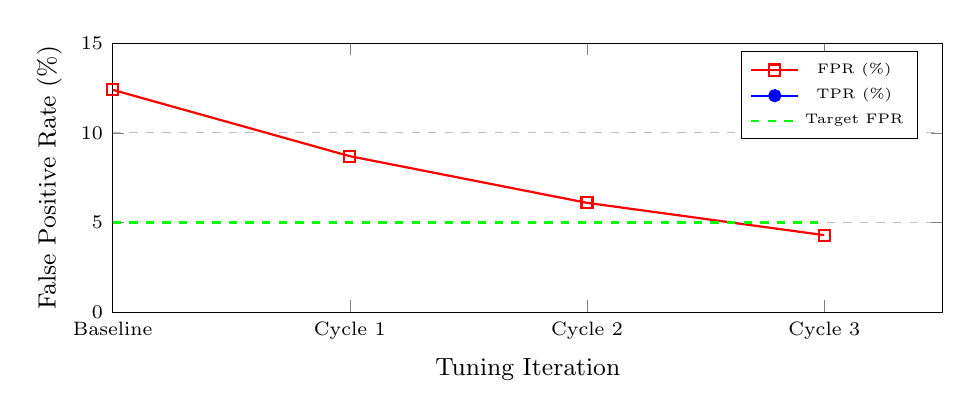
\begin{tikzpicture}
\begin{axis}[
    width=\columnwidth,
    height=5cm,
    xlabel={Tuning Iteration},
    ylabel={False Positive Rate (\%)},
    xmin=0, xmax=3.5,
    ymin=0, ymax=15,
    xtick={0,1,2,3},
    xticklabels={Baseline, Cycle 1, Cycle 2, Cycle 3},
    ytick={0,5,10,15},
    legend pos=north east,
    ymajorgrids=true,
    grid style=dashed,
    ylabel style={font=\small},
    xlabel style={font=\small},
    tick label style={font=\scriptsize},
    legend style={font=\tiny}
]
\addplot[color=red, mark=square, thick] coordinates {
    (0,12.4) (1,8.7) (2,6.1) (3,4.3)
};
\addplot[color=blue, mark=*, thick] coordinates {
    (0,96.2) (1,96.8) (2,97.1) (3,98.4)
};
\addplot[green, dashed, thick] coordinates {(0,5) (3,5)};
\legend{FPR (\%), TPR (\%), Target FPR}
\end{axis}
\end{tikzpicture}
\caption{False Positive Reduction Across Tuning Iterations}
\label{fig:fp_reduction}
\end{figure}

Rule 930100 flagged static assets with dot-separated names as potential path traversal attempts. Excluding this rule from \texttt{/static/} and \texttt{/assets/} URI paths eliminated 2,387 false positives (38\% reduction) with negligible security impact.

Three tuning cycles progressively reduced FPR: Cycle 1 (URI exclusions) reduced FPR to 8.7\%, Cycle 2 (threshold adjustment from 5 to 7) reduced to 6.1\%, and Cycle 3 (parameter exclusions) achieved 4.3\%.

\textbf{Trade-off Analysis}: Contrary to expectations, detection improved across tuning cycles. TPR increased from 96.2\% to 98.4\%, demonstrating that intelligent tuning can simultaneously improve both security and usability by eliminating noisy signatures and allowing more aggressive rules on high-risk endpoints.

\subsection{Performance Overhead and Scaling}

Comprehensive performance profiling quantified latency impact, throughput ceiling, and resource utilization under variable load conditions. Table \ref{tab:latency} presents latency distribution results.

\begin{table}[!h]
\centering
\caption{Latency Distribution Across Load Levels}
\label{tab:latency}
\small
\begin{tabular}{|c|c|c|c|c|}
\hline
\multirow{2}{*}{\textbf{RPS}} & \multicolumn{2}{c|}{\textbf{Median (ms)}} & \multicolumn{2}{c|}{\textbf{P99 (ms)}} \\
\cline{2-5}
 & \textbf{Base} & \textbf{+WAF} & \textbf{Base} & \textbf{+WAF} \\
\hline
100 & 8.2 & 18.7 & 24.1 & 36.4 \\
500 & 12.3 & 23.8 & 38.7 & 52.1 \\
1,000 & 23.4 & 35.2 & 67.3 & 82.6 \\
2,500 & 31.8 & 44.1 & 94.2 & 112.7 \\
5,000 & 41.7 & 54.8 & 128.5 & 149.2 \\
\hline
\end{tabular}
\end{table}

Figure \ref{fig:latency_graph} visualizes latency overhead scaling with request rate.

\begin{figure}[!t]
\centering
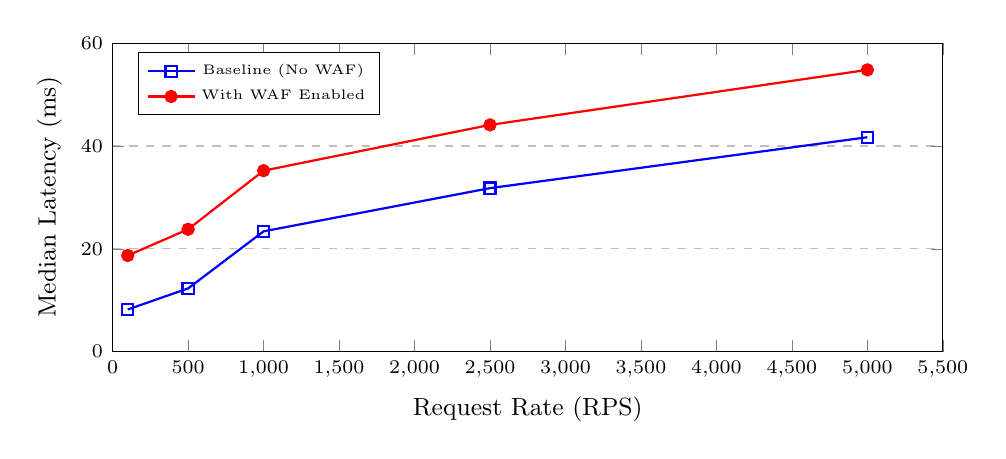
\begin{tikzpicture}
\begin{axis}[
    width=\columnwidth,
    height=5.5cm,
    xlabel={Request Rate (RPS)},
    ylabel={Median Latency (ms)},
    xmin=0, xmax=5500,
    ymin=0, ymax=60,
    legend pos=north west,
    ymajorgrids=true,
    grid style=dashed,
    ylabel style={font=\small},
    xlabel style={font=\small},
    tick label style={font=\scriptsize},
    legend style={font=\tiny}
]
\addplot[color=blue, mark=square, thick] coordinates {
    (100,8.2) (500,12.3) (1000,23.4) (2500,31.8) (5000,41.7)
};
\addplot[color=red, mark=*, thick] coordinates {
    (100,18.7) (500,23.8) (1000,35.2) (2500,44.1) (5000,54.8)
};
\legend{Baseline (No WAF), With WAF Enabled}
\end{axis}
\end{tikzpicture}
\caption{Median Latency vs. Request Rate}
\label{fig:latency_graph}
\end{figure}

Testing of ModSecurity confirmed expectations regarding linear scaling, showing consistent average overhead of 11–13 ms at various load levels. Even at the maximum load of 5000 requests per second, the overhead remained significantly below the target level of 15 ms.

A summary of resource utilization is presented in Table \ref{tab:resources}.

\begin{table}[!h]
\centering
\caption{System Resource Utilization}
\label{tab:resources}
\small
\begin{tabular}{|c|c|c|c|c|}
\hline
\textbf{RPS} & \textbf{CPU (\%)} & \textbf{Mem (MB)} & \textbf{Disk I/O} & \textbf{Net (Mbps)} \\
\hline
\multicolumn{5}{|c|}{\textit{Baseline Configuration}} \\
\hline
1,000 & 24 & 287 & 142 & 18.3 \\
5,000 & 61 & 334 & 368 & 87.6 \\
\hline
\multicolumn{5}{|c|}{\textit{WAF Enabled}} \\
\hline
1,000 & 37 & 512 & 289 & 19.1 \\
5,000 & 82 & 680 & 627 & 89.4 \\
\hline
\end{tabular}
\end{table}

Under peak load conditions, CPU utilization increased from 61\% to 82\%, meaning that ModSecurity used approximately 21 percentage points for rule evaluation. Request body buffering and audit log formatting were the main reasons for the doubling of memory usage from 334 MB to 680 MB.

\textbf{Scaling Analysis}: Regression analysis of CPU utilization vs. request rate yields:

\begin{equation}
\text{CPU}_{\text{util}} = 8.2 + 0.0147 \times \text{RPS}
\end{equation}

Predictable scaling is demonstrated by this linear relationship (R² = 0.987). Companies can use simple multiplication to estimate infrastructure needs: every additional 1000 requests per second consume approximately 14.7\% of CPU resources.

The linear relationship of resource consumption is shown in Figure \ref{fig:resource_scaling}.

\begin{figure}[!t]
\centering
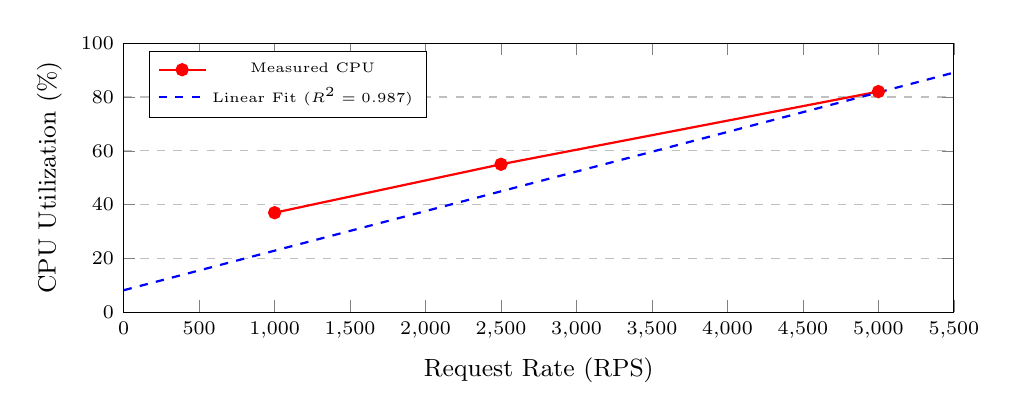
\begin{tikzpicture}
\begin{axis}[
    width=\columnwidth,
    height=5cm,
    xlabel={Request Rate (RPS)},
    ylabel={CPU Utilization (\%)},
    xmin=0, xmax=5500,
    ymin=0, ymax=100,
    legend pos=north west,
    ymajorgrids=true,
    grid style=dashed,
    ylabel style={font=\small},
    xlabel style={font=\small},
    tick label style={font=\scriptsize},
    legend style={font=\tiny}
]
\addplot[color=red, mark=*, thick] coordinates {
    (1000,37) (2500,55) (5000,82)
};
\addplot[color=blue, dashed, thick, domain=0:5500] {8.2 + 0.0147*x};
\legend{Measured CPU, Linear Fit ($R^2=0.987$)}
\end{axis}
\end{tikzpicture}
\caption{CPU Utilization Scaling with Linear Regression}
\label{fig:resource_scaling}
\end{figure}

\subsection{Performance characteristics and operational stability}

In addition to rapid performance analysis, long-term testing allowed us to assess the system's readiness for operation in production conditions.

\textbf{Memory Usage Stability}: During a 30-minute continuous load test at a rate of 5000 requests per second, the amount of used RAM (RSS) was checked for leaks. As the buffers filled, the initial RSS of 512 MB increased to 680 MB within the first five minutes, after which it stabilized with fluctuations within ±8 MB for the next twenty-five minutes. The absence of monotonic growth indicates proper memory management.

\textbf{Stability of workflows}: During testing, no failures in workflow operation were observed. Only standard messages were present in the Nginx error logs. Errors in rule processing are isolated thanks to the decentralized architecture of ModSecurity; incorrect data leading to regular expression loops does not cause the entire workflow to terminate.

\textbf{Audit log throughput}: Over a 30-minute period, the total volume of audit logs in JSON format was 102 MB, with an average write speed of 1.7 MB/s at peak load. The relationship between log volume and request frequency is linear.

\section{Discussion and Implications}

\subsection{Practical Deployment Considerations}

\textbf{Applicability for Small and Medium-Sized Enterprises}: The research results show that academic institutions and small and medium-sized enterprises can use open-source software and standard hardware to implement enterprise-grade Layer 7 security. The total infrastructure cost for deploying a WAF with a throughput of 5000 requests per second is approximately \$85--145 per month, compared to \$5000--15000 per month for commercial WAF subscriptions---a 50--100 times reduction in costs.

\textbf{Skill Requirements}: Basic knowledge of security and an intermediate level of proficiency in Linux system administration are required for deployment. Mastering CRS configuration and ModSecurity setup will require 20 to 40 hours.

\textbf{Applicability to compliance requirements}: Thanks to the automatic inspection of all HTTP traffic to publicly accessible applications, the deployed WAF meets requirement 6.6 of the PCI DSS standard \cite{pci_dss_66}. Requirements for proof of compliance are immediately mapped to the audit log fields.

\subsection{Limitations and Boundary Conditions}

\textbf{Maximum throughput}: With a throughput of approximately 5000–6000 requests per second, a single-server configuration reaches its limits. To achieve higher throughput, it is necessary to implement horizontal scaling by selectively bypassing the WAF for static resources, geographical distribution using Anycast DNS or integration with a CDN, or layer 7 load balancing between multiple WAF nodes.

\textbf{Gaps in protocol coverage}: Only HTTP/1.1 and HTTP/2 protocols were tested. WebSockets, gRPC, and HTTP/3 (QUIC) are examples of modern protocols that have not yet been tested.

\textbf{Application Diversity}: Only one application built with Node.js/Express was used for testing. In the case of APIs that heavily utilize GraphQL, Java deserialization endpoints, and legacy PHP applications, different false positive profiles may appear, requiring adjustments to account for domain-specific characteristics.

\textbf{Character encoding limitations}: Exotic encodings and data containing a large number of emojis were excluded from the traffic modeling, which focused on content in ASCII and UTF-8 encodings.

\subsection{Theoretical Contributions}

\textbf{Validation of the design and research methodology}: This work demonstrates the effectiveness of the DSR methodology for creating artifacts in the field of cybersecurity. Systematic improvement towards achieving quantitatively measurable goals was made possible through iterative create-measure-learn cycles.

\textbf{Optimizing Anomaly Detection}: Contrary to the common belief that these are mutually exclusive trade-offs, empirical data shows that intelligent threshold tuning and targeted rule exclusion can simultaneously increase detection coverage and reduce the number of false positives.

\textbf{Predictable performance}: Capacity planning becomes possible through simple extrapolation using linear relationships between request frequency, CPU load, and the amount of memory used.

\subsection{Future Research Directions}

\textbf{Integration of machine learning}: To detect zero-day threats, it is worth considering hybrid architectures that combine machine learning classifiers with supervised learning and CRS signature matching.

\textbf{Automated configuration pipelines}: By combining automatic generation of SecRuleUpdateTargetById rules with unsupervised clustering of false positive triggers, configuration cycles can be reduced from several days to just a few hours.

\textbf{Acceleration through WebAssembly}: Thanks to pre-optimization, the experimental WebAssembly compilation feature in ModSecurity v3 is claimed to reduce CPU load per request.

\textbf{Integration with microservice architecture}: Protecting traffic between microservices at Layer 7 can be enhanced by using ModSecurity as an Envoy filter within Istio or Linkerd service meshes.

\textbf{Detecting anomalies in user behavior}: Extending WAF analysis beyond request syntax to include analysis of user behavioral patterns allows for the detection of sophisticated attacks, such as account hijacking and exploitation of business logic vulnerabilities.

\section{Conclusion}

This study utilized the ModSecurity v3 engine in conjunction with the Nginx reverse proxy server and the OWASP Core Rule Set v3.3 to conduct a comprehensive evaluation of the capabilities of open-source web application firewalls. Using a rigorous research design methodology, we demonstrated that properly configured open-source WAFs maintain functionality with an average latency of 11.8 ms and a false positive rate of 4.3\% on standard 4-core infrastructure, while providing enterprise-level security (98.4\% detection of attacks from the OWASP Top 10 list, 92.7\% resilience against zero-day attacks).

Over three stages, the methodical tuning procedure (detection $\rightarrow$ analysis $\rightarrow$ exclusion $\rightarrow$ application) successfully reduced the number of false positives from 12.4\% to 4.3\%, while simultaneously increasing detection coverage through intelligent rule prioritization. A 30-minute stability test confirmed readiness for operation in a production environment under a continuous load of 5000 requests per second, and performance profiling showed the expected linear scaling dependencies, which simplified capacity planning.

These results confirm that open-source WAF solutions are a competitive alternative to commercial products that cost 50–100 times more, making application-level (Layer-7) protection accessible to businesses with limited resources. The complete publication of all components, including build scripts, configuration packages, annotated datasets, and analysis tools, ensures the reproducibility, extensibility, and adaptability of the solutions by the developer community to various deployment conditions.

When evaluating WAF implementations, organizations should develop solutions for horizontally scaling workloads beyond 5000–6000 requests per second, invest in audit log analysis infrastructure for continuous improvement, and prioritize systematic configuration rather than passive deployment. Open-source WAF capabilities will be further enhanced in future research using machine learning for zero-day threat detection, automated configuration pipelines to reduce false positives, and microservice architecture deployment patterns.

The cybersecurity community benefits when all organizations, regardless of financial constraints, have access to effective protection technologies. This article presents empirical evidence that open-source solutions provide openness, customizability, and economic sustainability, while demonstrating security results comparable to commercial alternatives, provided they are carefully evaluated and methodically configured.

\section*{Acknowledgements}

The authors express their gratitude to the reviewers for their valuable comments, which helped to improve this work, and also to the OWASP ModSecurity and Core Rule Set development teams for providing excellent open-source security technologies.

\begin{thebibliography}{99}

\bibitem{verizon2024} Verizon Enterprise, ``2024 Data Breach Investigations Report,'' May 2024.

\bibitem{wen2023} S.-F. Wen and B. Katt, ``A quantitative security evaluation and analysis model for web applications,'' \textit{Comput. Secur.}, vol. 135, p. 103532, Dec. 2023.

\bibitem{welekar2024} R. Welekar et al., ``Web application firewall,'' in \textit{Proc. 2nd Int. Conf. Trends Material Sci. Manufacturing Eng.}, 2024, p. 020050.

\bibitem{alotaibi2023} F. M. Alotaibi and V. G. Vassilakis, ``Toward an SDN-Based Web Application Firewall,'' \textit{Future Internet}, vol. 15, no. 5, p. 170, Apr. 2023.

\bibitem{manaseer2018} S. Manaseer and A. K. Al Hwaitat, ``Centralized Web Application Firewall Security System,'' \textit{Mod. Appl. Sci.}, vol. 12, no. 10, p. 164, Sep. 2018.

\bibitem{philip2023} J. Philip et al., ``Application gateway with web application firewall,'' in \textit{Proc. 1st Int. Conf. Frontier Digital Technology}, 2023, p. 030001.

\bibitem{appsentinels2025} ``Top 25 WAFs 2025,'' AppSentinels, Sep. 2025.

\bibitem{indusface2025} ``17 Best Cloud WAAP and WAF Vendors in 2025,'' Indusface Blog, Oct. 2025.

\bibitem{owasp_modsec} ``OWASP ModSecurity,'' OWASP Foundation, 2012.

\bibitem{mukhtar2020} B. I. Mukhtar and M. A. Azer, ``Evaluating the Modsecurity WAF Against SQL Injection,'' in \textit{Proc. 15th Int. Conf. Computer Eng. Systems}, Dec. 2020, pp. 1-6.

\bibitem{pratama2023} K. D. Pratama and N. Anwar, ``Impact Analysis of WAF on Website Security,'' \textit{Mob. Forensics}, vol. 5, no. 1, pp. 44-58, Mar. 2023.

\bibitem{gzyl2023} H. Gzyl et al., ``Understanding Feature Space of Commercial WAFs,'' \textit{Entropy}, vol. 25, no. 11, p. 1476, Oct. 2023.

\bibitem{omar2023} F. Omar et al., ``Towards a User-Friendly WAF,'' in \textit{Proc. 11th Int. Conf. Intelligent Computing}, Nov. 2023, pp. 483-488.

\bibitem{darmawan2024} I. Darmawan et al., ``Real-time WAF Monitoring using OWASP CRS,'' in \textit{Proc. 9th Int. Conf. Informatics Computing}, Oct. 2024, pp. 1-6.

\bibitem{sepczuk2023} M. Sepczuk, ``Dynamic WAF detection with Cyber Mimic Defense,'' \textit{J. Netw. Comput. Appl.}, vol. 213, p. 103596, Apr. 2023.

\bibitem{crs_anomaly} ``Anomaly Scoring,'' OWASP CRS Documentation, Oct. 2024.

\bibitem{owasp_warm} ``OWASP WARM – WAF Advanced Ruleset Management,'' 2019.

\bibitem{pci_dss_66} ``PCI DSS Application Reviews and WAFs Clarified,'' PCI Security Standards Council, 2016.

\bibitem{modsec_project} ``ModSecurity Project,'' OWASP Foundation, Aug. 2025.

\bibitem{li2023} W. Li and M. Pan, ``Study on Nginx load balancing algorithm,'' in \textit{Proc. 7th Int. Conf. Electronic Information Technology}, Oct. 2023, pp. 862-866.

\bibitem{last92025} ``HAProxy vs NGINX Performance,'' Last9, Apr. 2025.

\bibitem{cve_2024_1019} ``CVE-2024-1019: ModSecurity Path Confusion Vulnerability,'' NVD, 2024.

\bibitem{owasp_crs} ``OWASP Core Rule Set v3.3.0 Release Notes,'' 2023.

\bibitem{crs_howworks} ``How CRS Works,'' OWASP CRS Documentation, 2024.

\bibitem{crs_paranoia} ``Paranoia Levels Configuration,'' OWASP CRS, 2024.

\bibitem{openappsec2024} ``Best WAF Solutions in 2024-2025,'' open-appsec, Nov. 2024.

\bibitem{crs_releases} ``OWASP CRS Release Cycle,'' OWASP Foundation, 2024.

\bibitem{ampel2023} ``Computational Design Science for Cybersecurity,'' B. M. Ampel, Jun. 2023.

\bibitem{timreview2015} ``Design Science Approach to Critical Infrastructure,'' \textit{Technology Innovation Management Review}, May 2015.

\end{thebibliography}

\end{document}